\subsection{Laue-Aufnahme}
\begin{figure}
\centering
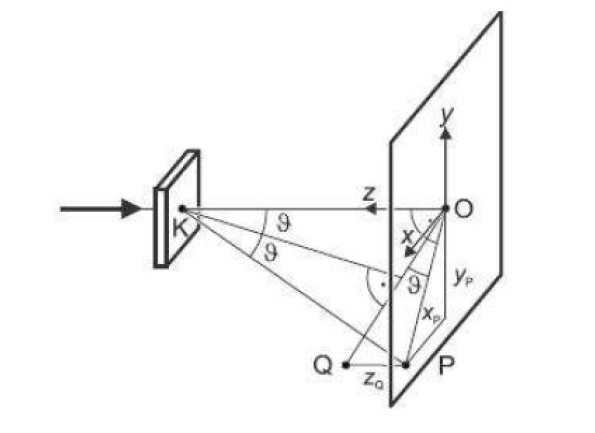
\includegraphics[scale=0.5]{data/laue/th_laue.png}
\caption{Konstruktion des reziproken Gittervekors\cite{praktikumsheft}}
\label{fig:laue_th}
\end{figure}

In Abb. \ref{fig:laue_th} ist die Situation bei der Laue-Aufnahme dargestellt (Wir verwenden das Koordinatensystem, so wie es in der Abb. \ref{fig:laue_th} angegeben ist). Röntgenstrahlung fällt von links parallel zur z-Achse auf den Kristall ein. Es wird an den Gitterpunkten gestreut. Geht man von einem kubischem Gitter, dessen Achsen in x-,y- und z-Richtung verlaufen, aus, dann kann man jeden Vektor $\vec{R}$ von einem Gitterpunkt zu einem anderen eindeutig darstellen durch ($a_0$ ist der Abstand zweier Gitterpunkte):
\begin{align*}
\vec{R} &= n_1\vec{a}_1 + n_2\vec{a}_2 + n_3\vec{a}_3 & n_1,n_2,n_3 \in \mathbb{Z}\\
	\vec{a}_1 &= a_0\vec{e}_x\\
	\vec{a}_2 &= a_0\vec{e}_y\\
	\vec{a}_3 &= a_0\vec{e}_z\\ 
\end{align*}

Weiterhin sind die reziproken Gittervektoren im Falle eines kubischen Gitters definiert durch:
\begin{align*}
\vec{G} &= h\vec{b}_1 + k\vec{b}_2 + l\vec{b}_3 & h,k,l \in \mathbb{Z}\\
\vec{b}_i &= \frac{2\pi}{a_0} \vec{e}_i
\end{align*}

\begin{figure}
\centering
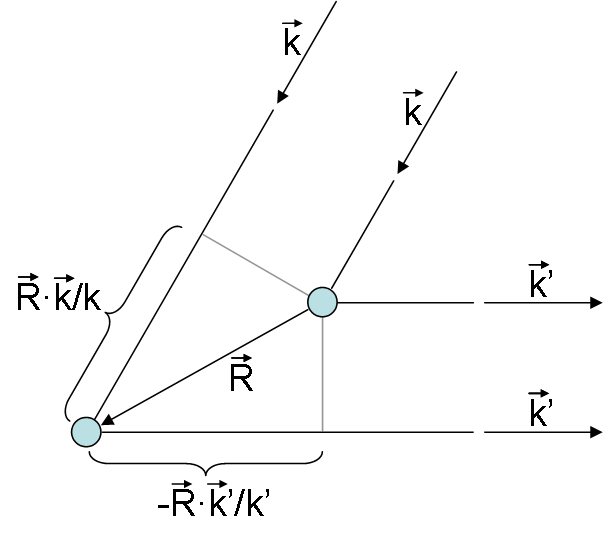
\includegraphics[scale=0.75]{data/laue/Laue-Bedingung.png}
\caption{Gangunterschied bei der Streuung am Gitter\cite{wiki_laue_bed}}
\label{fig:laue_bed}
\end{figure}

Fällt Röngtenstrahlung in Richtung $\vec{k}$ auf den Kristall ein und wird in Richtung $\vec{k}'$ gestreut (siehe Abb. \ref{fig:laue_bed}) so ergibt ein Gangunterschied zwischen der Streuung an verschiedenen Streuzentren. 

Die Lauebedingung für konstruktive Interferenz lautet, dass $\Delta \vec{k} = \vec{k}'-\vec{k}$ ein reziproker Gittervektor ist \cite{wiki_laue_bed}:
\begin{align*}
\vec{G} = \Delta \vec{k} &= h\vec{b}_1 + k\vec{b}_2 + l\vec{b}_3
\end{align*}

Sieht man einen Reflex (also einen Punkt, bei dem konstruktive Interferenz stattfindet) auf dem Schirm, so kann man diesem die Koordinaten $x\ind{Q}$ und $y\ind{Q}$ zuweisen. Es gilt:
\begin{align*}
(x\ind{Q}, y\ind{Q},-L) &\sim \vec{k}'\\
(x\ind{Q}, y\ind{Q},-L) &= \beta \vec{k}'\\
(x\ind{Q}, y\ind{Q}) &= \alpha (h,k) & \text{da}\;\;(k\ind{x}',k\ind{y}') \sim (h,k),
\end{align*}
wobei $\alpha, \beta$ zwei reelle Zahlen sind.

Nun muss man nur noch $l$ bestimmen. Dies bekommt man aus der Bedingung, dass $\Delta\vec{k} = \vec{k}' -\vec{k}$:
\begin{align*}
\vec{k} &= -k\vec{e}\ind{z} & \text{nach Abb. \ref{fig:laue_th}}\\
\Delta\vec{k} &= h\vec{b}_1 + k\vec{b}_2 + l\vec{b}_3 = \frac{2\pi}{a_0} (h, k, l)\\
\vec{k}' &= \vec{k} + \Delta\vec{k} = -k (0,0,1) + \frac{2\pi}{a_0} (h,k,l)\\
\vec{k}' &= \frac{1}{\beta} (x\ind{Q},y\ind{Q},-L) &\Rightarrow \alpha = \beta \frac{2\pi}{a_0}\\
\frac{-L}{\beta} = k\ind{z}' &= -k +\frac{\alpha l}{\beta} = -k + \frac{z\ind{Q}}{\beta} & z\ind{Q} := \alpha l\\
z\ind{Q} &= k\beta - L\\
\end{align*}

Da man elastischer Streuung ausgeht, gilt $|\vec{k}| = |\vec{k}'|$: 
\begin{align*}
k\beta &= |\beta\vec{k}'| = \sqrt{(x\ind{Q}, y\ind{Q},-L)^2} = \sqrt{x\ind{Q}^2 + y\ind{Q}^2 + L^2}\\
z\ind{Q} &= k\beta - L = \sqrt{x\ind{Q}^2 + y\ind{Q}^2 + L^2} - L
\end{align*}

Nun ersetzt man noch $(x\ind{Q}, y\ind{Q}, z\ind{Q}) = \alpha (h,k,l)$ und erhält:
\begin{align*}
z\ind{Q} &= \sqrt{x\ind{Q}^2 + y\ind{Q}^2 + L^2} - L\\
(z\ind{Q}+L)^2 &= x\ind{Q}^2 + y\ind{Q}^2 + L^2\\
(z\ind{Q}+L)^2 &= x\ind{Q}^2 + y\ind{Q}^2 + L^2\\
z\ind{Q}^2+2z\ind{Q}L &= x\ind{Q}^2 + y\ind{Q}^2\\
\alpha^2 l^2+2\alpha l L &= \alpha^2 h^2 + \alpha^2 k^2\\
\alpha l^2+2 l L &= \alpha h^2 + \alpha k^2
\end{align*}  

Durch umstellen kommt man zu der Formel:
\begin{align}
\alpha &= \cfrac{2lL}{h^2 + k^2 - l^2}
\label{eq:alpha}
\end{align} 